\documentclass{sig-alternate-05-2015}

\RequirePackage[]{silence}
\WarningsOff[hyperref]
\usepackage {hyperref}

\begin{document}
% Copyright
\setcopyright{acmcopyright}

% DOI
\doi{10.475/123_4}

% ISBN
\isbn{123-4567-24-567/08/06}

%Conference
\conferenceinfo{WEA '16}{Copenhagen, 2016}

% --- Author Metadata here ---
\conferenceinfo{WOODSTOCK}{'97 El Paso, Texas USA}
% --- End of Author Metadata ---

\title{Bootstrapping a Software Ecosystem for Accelerating Second Language Acquisition}

% Alternative Titles
% (Growing a) Learning Software Ecosystem Based on Ubiquitous Monitoring and Adaptive Tutoring
% Lessons Learned while Growing a Learning Software Ecosystem
% How to Tame a Dragon - How to Grow an Ecosystem 
% A Platform for Growing a Learning Software Ecosystem
% Lessons Learned While Bootstrapping a Learning Software Ecossytem

\author{
Mircea F. Lungu \\
       \affaddr{SEARCH @ Johan Bernoulli Institute}\\
       \affaddr{University of Groningen}\\
       \affaddr{Netherlands}\\
       \email{i@mir.lu}
}

% \date{30 July 1999}

\maketitle
\begin{abstract}

Learning the vocabulary of a new language is a very slow and time consuming process which can take many years of dedicated study. 

In this paper I present the idea of an ecosystem which by monitoring the reading activities of a learner can build a model of their evolving knowledge and steer their future reading and studying sessions in such a way as to accelerate the speed with which they acquire new vocabulary. 

I describe a high-level architecture of the underlying platform dubbed Zeeguu, and exemplify some of the lessons learned while bootstrapping the ecosystem with several applications that complement each  other but are joined in the aim of accelerating vocabulary acquisition in a second language. 

\end{abstract}


\newcommand{\Lesson}[1]{ \vspace {0.3cm} \hrule \vspace{0.2cm} {\bf #1} \vspace{0.2cm} \hrule \vspace{0.3cm}}

\keywords{software ecosystems; software design; human-computer interaction; applied linguistics;}

\section{Introduction}

At any given moment millions of people are learning the vocabulary of a new language. The first steps in the acquisition of the new language are usually full of enthusiasm, but often the learner gives up once he realizes the magnitude of the task.

Indeed, once a learner has acquired the basic vocabulary of a foreign language, they are still many thousands of words away from actually mastering the new language. To improve their vocabulary they must constantly expose themselves to contexts in which the learned language is used at a level that is not too difficult but not too easy either -- or how some psychologists are calling this, {\em they must study in the zone of proximal development}. Reading language textbooks is the traditional approach but more often than not textbooks being written for everybody are uninteresting for anyone.

Amazon has made a first step towards allowing the learner to read engaging texts by integrating translations and basic vocabulary exercises with their proprietary eBook reader device. Besides the limitations of being locked to a given dvice, this solution suffers also from the fact that the words being learned are locked in by Amazon. We will see later that this limits the possibilities of accelerating the speed with which vocabulary acquisition happens.

Another solution that the readers have is using Google Translate on the web. However, just as with Amazon, the translations that the user makes online are as of middle of 2016 not available outside the Google ecosystem. Thus the possibility of other applications benefiting from the knowledge of what the user is learning at the moment is also absent.

On the side of vocabulary rehearsal applications a plethora of solutions most of them being its own data silo. 



\section {A Learning Ecosystem}

To address the disadvantages of the locked down nature of the existing infrastructures, we propose as a solution an open ecosystem that will combine their advantages while avoiding their limitations. The ecosystem should be built on the following principles:

\begin{itemize}

	\item The learners should be able to read anything that they find interesting. Ubiquitous translations should be offered while the context in which the translation request was made will be saved to the learners' profile. The context can be useful for further personalized exercises. To cover as many reading contexts as possible, it should be easy for new reading applications to join the ecosystem.

	\item An evolving model of the current state of the knowledge of the learner should be built by tracking and observing the users' interactions with foreign texts. The applications in the ecosystem that want to, should have access to this model.

	\item Intelligent agents should recommend reading and exercises that maximize the likelihood of encountering the most important learned words at the optimal times for every learner.

	\item The system should be open for any type of application that wants to contribute to it, either academic or industrial. The application would be able to make use of the information in the user profile as long as they contribute back to the ecosystem. 

\end{itemize}


\newpage
\section {The Zeeguu Platform}

A prototype of a learning ecosystem as described in the previous section is currently being bootstrapped at the Universities of Bern and Groningen. It is growing around an open platform dubbed Zeeguu. 

Figure \ref{fig:architecture} presents a very simplified version of the Zeeguu platform and ecosystem although it should be noted that the diagram is general enough for representing any learning ecosystem. The main components of the architecture in the case of Zeeguu are:

\begin{figure}[h!]
	% \centering
	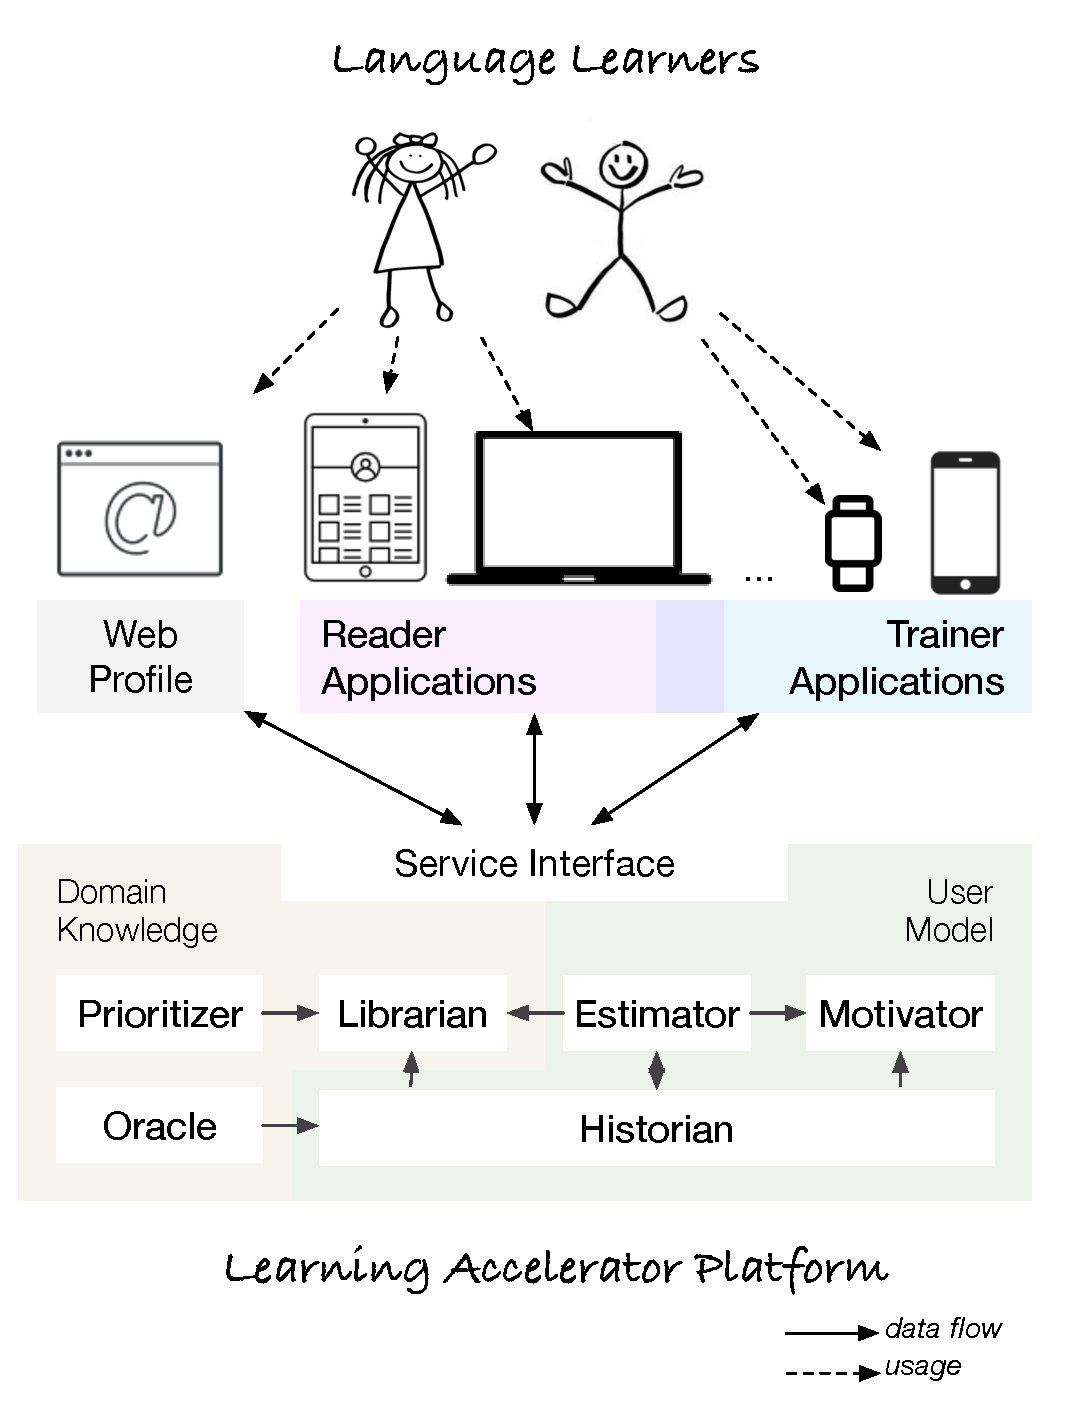
\includegraphics[width=\linewidth]{zeeguu-architecture.pdf}
	\caption{A very high-level view of the architecture of the Zeeguu ecosystem}
	\label{fig:architecture}
\end{figure}


\begin{itemize}
	
	\item {\bf Reader Assistants} 
	support reading any kinds of materials in foreign languages. The reader applications must have two properties in common: 
		1) they should make it very convenient for the user to obtain translations for the texts he encounters in the foreign language. 
		2) they should track every event that provides a hint to the current user knowledge. In particular, every word that is being translated by the user indicates his lack of knowledge with respect to that particular word, and every word that is not being translate by the user indicates their knowledge of that word. 
	
		\item {\bf User Model Store} 
		% User Model Database
		% User Model Registry
		% User Model Store
		is a core component of the learning ecosystem since it stores and orchestrates the exchange of information about the current and historical knowledge of the user. It needs to have several components, including: 

		\begin{itemize}

			\item The {\bf Interaction Historian} represents a centralized data warehouse that stores all the interactions of a learner with texts in the foreign language that are mediated by the Reader applications.

			\item The {\bf Knowledge Estimator} tries to approximate the current knowledge of the user based on the interaction history, and the feedback received from the Trainer agents, and other types of information that are available about the user

			\item The {\bf Oracle} is an agent which decides what are the most important items to be studied next by the learner. 
			% We envision multiple oracle implementations competing with each other

		\end{itemize}


	\item {\bf Trainer Agents} support the learner in practicing the vocabulary and must interact with the user model. A trainer application can request from the user model store information on which words are to be learned by the learner. But a trainer application must also provide back to the central user model information about how well the learner behaves with respect to a given word, otherwise this information will be lost. 
	
	% Two types of trainer agents are: 
	% \begin{itemize}
	% 	\item Librarians --  can recommend articles to read, music to listen to, movies to watch, etc.
	% 	\item Coaches -- which provide exercises for learning 
	% \end{itemize}
	% - Librarians -- 
	% - Coaches -- which use exercises to help the learner rehearse 


	
\end{itemize}

Note that as the Figure \ref{fig:architecture} suggests, the Reader Assistants and Trainer Agents need not be disjoint applications, but one application could provide both.

It might appear intuitive for the reader that the more contexts in which the reader is supported by applications from the ecosystem, the better the knowledge model of that learner that can be built, and the better the user experience. Such a learning ecosystem can thus present a network effect where its value will increase more than linear with the number of applications that contribute to it.

% Somewhere, we still have to discuss the question of: 
% - How are we going to maintain this ecosystem? who will provide the data storage and translation facilities for the long run? 
% - What are the incentives for new players to join the ecosystem?
% - ... 



\section {Bootstrapping the Ecosystem}

In this section we present in chronological order several of the applications that have been added to the ecosystem during the recent years. Where appropriate we discuss lessons learned for the platform developer who hopes to become future ecosystem owner. 

\subsection {The API, The App, and The Extension}
The first milestone was releasing in 2013 a prototype version with three main components: 

\begin{itemize}
	\item One Reader Assistant implemented as a Chrome extension. It allows a learner to read any text on any website if they are using Chrome as a Browser\footnote{The extension is available at: \url{https://zeeguu.unibe.ch/chrome}}. 

	\item An Initial User Model exposed via a REST API  \cite{Lung16zeeguu}. 

	\item A web application\footnote{The web application is available at \url{https://zeeguu.unibe.ch}} responsible with account management, and a very basic interface to show a learner's reading history. 

	\item One very simple trainer agent to be found inside of the web application which asks the learner to recognize a given word within its context. The words and contexts are selected from the past readings of the learner.

\end{itemize}

At the time, the web application, and the REST API were deployed together on the same serve as a Python-based applications and the separation between them was not well enforced. This came to hunt us later when we discovered that as we were extending the REST API for other applications, we duplicated functionality that was already existent in the Web Application since the Web Application was accessing the DB directly instead of going through the API.

%One lesson that we learned based on this experience is that: 

\Lesson {It is desirable to treat even the internal applications as one plans to treat future third-party applications. They represent a test case for functionality, and in the long run this will avoid duplicated code.}

The Chrome extension as a reader assistant posed two main limitations: 
	1) not everybody is reading his foreign language texts on their computer and,
	2) some users are circumspect when it comes to installing third-party browser extensions.
To address these problems, we decided to add new readers to the ecosystem.



\subsection {A Reader for Android}

The Zeeguu Reader for Android was implemented as a bachelor project by Schwab\cite{Schw16thesis}. The application is written in Java and functions as an RSS feed reader that relies on the Feedly API to manage user's reading interests.

The architecture of the application made a clear distinction between two components: 

\begin{enumerate}
	\item The Zeeguu Android Library would ease the communication with the REST API and was released as a separate open-source component\footnote{\url{https://github.com/linusschwab/zeeguu-android-library}} and 
	\item the actual Android  application. 
\end{enumerate}

The separation has proven to be a good design choice since a second Android application -- a Dictionary \cite{Gieh15a} which was implemented by another student could readily benefit from the API component.

At the same time, the fact that the dictionary was a different application was also a problem. During usability studies we learned that at least some of the users found it inconvenient to have two applications installed. They would have preferred to have a single application instead. 

\Lesson {When growing a software ecosystem, it pays to study whether fusing multiple applications in a single one could increase adoption.}

One of the features of the Android News Reader was ranking news items based on their difficulty with respect to the current estimated knowledge of the learner. However, since such an algorithm would very likely be required for other applications in the ecosystem, we decided to move this functionality in a separate component on the server and expose it using an API. 

\Lesson {In learning ecosystems, functionality that would benefit multiple applications, and especially that functionality which regards learner modeling, will tend to migrate towards a central point}

The Android RSS Feed Reader relies on a third party API from Feedly to allow a reader to register to and track news feeds. This turned out to be very cumbersome for learners since they required to create a new account to a different service, before using the Reader Application.


\subsection {A Reader for iOS}

A news and blog reader for iOS devices has been implemented as a bachelor thesis by Oosterhof \cite{Oost16reading}. The application written natively in Swift eliminates the explicit dependence on third party services like Feedly. Instead the burden of extracting feed information from pages, and monitoring news in feeds has been moved into a separate agent inside of the User Model. Correspondingly the REST API grew with new functionality.

The architecture of the iOS application, made again, as in the case of Android, a clear separation between a component which was to interact with the API\footnote{\url{https://github.com/mircealungu/zeeguu-ios-library}} and the actual GUI of the application. 

For every new language the developer had to handwrite a new API interface that would communicate with the user model. This made us realize the missed opportunity of automatically generating the APIs for different languages. However, as far as we are aware, no such generator exists for the Python technology stack used. 

\Lesson {Since adoption is eased by providing APIs in different languages, the platform developer should consider using technologies that enable the automatic generation of APIs for various languages.}


\subsection {Smartwatch Trainer}

According to current estimates, the wearable market\footnote{Which includes fitness trackers and smartwatches, so the number of smartwatches is likely smaller} will pass 111 million shipped devices in 2016, up from 80 million shipped in 2015. The ease with which a user can consult his smartwatch makes it an interesting platform for a learning strategy called micro-learning known for quickly closing skill and knowledge gaps  \cite{Dear12}. Having a trainer on the smartwatch would make it easy for the learner to take advantage of dead moments during the day (e.g. waiting for the elevator) and use them for learning.

A trainer, dubbed {\em Time to Learn}, was implemented for the Gear S2 smartwatch by Haan and Nienhuis\cite{Nien16time}. The Gear S2 device runs on the Tizen mobile operating system and applications for it can be implemented using HTML5 and Javascript.

To support micro-learning, the information on the smartwatch should be readily available when a learner looks at the watch. Thus, Time to Learn divides the watch face in two: the top half presents the usual watch information, while the bottom part represents a word recognition challenge for the learner. The word to be displayed is retrieved from the user model API recommendations. 

After every challenge, the learner provides feedback on whether he knew a given word or not. This feedback is sent back to the user model so it can be used in the future by the knowledge estimator. 

What we discovered was that, on the server, the knowledge estimation module has to take into account the existence of the smartwatch events explicitly. This forces the knowledge estimator module to be aware of the individual applications in the ecosystem, or at least of some of them -- in our case, the trainer agents. Theoretically, if the knowledge estimator would be fully implemented with machine learning technologies, it could be agnostic about the existence of the indiviudal trainers. However, this direction needs to be explored further.

\Lesson {As long as a core component in a learning ecosystem needs to take decisions based on differentiating individual signals from different applications, it is impossible to hide from it the existence of different types of applications.}




\section {Reflections}

It is still not clear when and if this ecosystem will 
take on a life on its own. Until now, all the 
applications that were added, have been in one way
or another supported by the creator. The challenge
of incentivizing external players and
to defining policies that will benefit all the 
players still remains \cite{Jans09agenda}.


Also, this is not the first ecosystem that aims to track 
the interactions of a user with data and build a better 
user model based on this; many commercial companies do it too. 
However, the goals of these companies are usually economic, 
while the goal of our ecosystem would be research and education.

It would seem thus, that since profit is not the main
goal of such an ecosystem, we should be confronting
with different problems than those enterprises where 
profit is critical. However, the economical 
sustainability of the platform when hosted in academia
is still an open question. The hosting costs of the 
core components are at the moment not significant 
but they could become large in the eventualily of 
a massive growth.


One way to do this would be to unequivocally show 
the benefits it brings to the learners. Based on 
early user studies and the feedback we received 
from individual applications we can say that such
an ecosystem shows promise. But more work has to 
be done for this. 

% One other aspect that has not been discussed here
% but which will have to be dealt with at some point 
% is the privacy issue. How can we make sure that 
% private information about a reader does not leak
% between applications. 

Finally, there is no claim or expectation that the 
lessons derived here hold beyond the given case study. It 
might be and it is our hope that they can be of 
use for other learning ecosystem development
projects, but until more such results 
are published, this remains to be seen.



% - how to insure privacy? should everything in the profile be visible for all the apps?




\section{Conclusion}

The paper presents a proposed architecture and reports
several lessons learned while building a platform that
aims to support learning software ecosystem. 
The ecosystem is designed for accelerating second language
vocabulary acquisition but probably such an approach can 
be extended to other types of learning. 

\vspace{0.5cm} 
\noindent {\bf Acknowledgements} The author would like to thank
Jens Knodel and Anca Lungu for feedback on early versions 
of this paper. 

\newpage

\bibliographystyle{IEEEtran}
\bibliography{mir-biblio/aslan,mir-biblio/eco}



\end{document}
